\documentclass[a4paper]{article}
\usepackage{makeidx}
\usepackage{listings}
\usepackage{graphicx}
\usepackage{hyperref}

\lstset{frame=none, numbers=none}
\lstMakeShortInline[flexiblecolumns=false, basicstyle=\small];

\title{Proof Assistant Help}
\author{Declan Thompson}
\date{Version 1.4\\
			\today}
			
\makeindex
\begin{document}
\maketitle

\tableofcontents

\section{Introduction}
This is the help file for the Proof Assistant natural deduction proof creator. This document is intended to explain basic usage of the application from a user's point of view. For information on how to implement changes, bugfixes or additions, see the file \texttt{proofassistantdoc}, which endeavours to explain the code. This document will cover basic usage, advanced usage and the more experimental features. There is also a section on input style to ensure correct parsing of inputs.

But first I will explain the background assumed for the full use of this application.

\subsection{Assumed Background}
This application assumes the user is familiar with (or at the very least is learning) the style of Natural Deduction logical proof taught in Philosophy 222 ``Intermediate Logic'', a course at the University of Auckland. No attempt has been made to explain how these proofs should be conducted.

The export options have been designed to accommodate a variety of users, however the {\TeX} output option has (clearly) been targeted at the {\LaTeX} user. This was the first output option implemented and requires two \texttt{.sty} files - \texttt{ndproof.sty} and \texttt{mylogicv03.sty}. The acquisition of these files is a task left to the reader. The usage of \texttt{ndproof.sty} assumes an understanding of {\LaTeX} code, and help for it can be found in the \texttt{ndproofdoc} document.

\subsection{Application Scope}
The proof assistant does not attempt to be an automatic proof solver. Rather, it is a means to solving a proof. The application simply replicates the layout used in pen-and-paper Natural Deduction proofs, presenting the user with the rules they may choose to proceed with. It is like proving a sequent on paper, but with someone else doing the writing for you.

Included are the introduction and elimination rules for conjunction, disjunction, implication, equivalence, negation, the existential quantifier, the universal quantifier, identity (including identity boxes), box and diamond (from Modal Logic) and @, nominal and self-reference (from Hybrid Logic). Further available rules include double negation, induction, justifying from an identical line and a simple, limited implementation of second-order logic. The user also has the ability to display the Robinson Arithmetic axioms, and to set custom axioms. Furthermore, the ability to use general equational reasoning has been implemented.

The application has the ability to export proofs to a variety of outputs including {\TeX} code, plain text and image formats. Proofs can be saved/opened as editable or uneditable files.

\section{Basic Usage}
\label{sec:BasicUsage}
This section documents the basic features of the Proof Assistant. It is divided into four sections: program layout, completing a proof, export and further features.

\subsection{Program Layout}
\label{subsec:ProgramLayout}
To begin with, we will consider the layout of the program, and look at some important dialogs.

Upon opening the Proof Assistant, you will be presented with the main window, or \emph{Proof Frame}\index{Proof Frame}. This has a main menu along the top and a status bar at the bottom. The main blank area is called the \emph{Proof Panel}. You can resize the Proof Frame, but it will not go below minimum dimensions.

\subsubsection{The Proof Panel}
The Proof Panel\index{Proof Panel} is located in the main content area of the Proof Frame. This is where you will work through the proof itself. The proof is displayed here, as are the rules you may wish to use.

\subsubsection{The Rule Palette}
The \emph{ruleset} governs the rules available to you for use in the proof. The current ruleset is displayed in the status bar. To change the ruleset, open the \emph{Rule Palette}\index{Rule Palette} by clicking on the name of the current ruleset (in the status bar) or under \emph{Options} in the main menu.

The Rule Palette is divided into two areas. At the top, you can select from any of the predefined presets, or save the current ruleset to a new preset. Below are a series of task panes. Each of these contains checkboxes corresponding to rules. To activate or deactivate a rule, simply select or deselect the appropriate checkbox.

\subsubsection{The Arity List}
\label{subsubsec:ArityList}
If you are using functions in your proof, you will want to check (and possibly change) the arity list\index{Arity List}. This list holds the arity of every symbol. Any symbol not on the arity list will be treated as a propositional variable or predicate symbol. If you wish to use a symbol, say ;m;, as a term, add ;m0; to the arity list. To use ;m; has an \emph{n}-ary function, add ;m;\emph{n} to the list (so long as \emph{n} is indeed an integer). If ;m; is already a term, but you want to use it as a propositional variable, add ;m; to the list and it will be removed.

Predicate Symbols should not be added to the arity list. The arity of a predicate symbol does not need to be specified as the information is not used.

Using the correct arities is important, as they affect how lines are displayed and how identity rules are applied.

The arity list can be accessed in two ways. From the \emph{New Proof} dialog (documented below), you can add to the arity list via the \emph{Quick change arities} text field. Alternatively, you can open the \emph{Settings}\index{Settings} dialog from \emph{Options} or by clicking the word \emph{Arities} in the status bar. From here, you can set arities.

To change arities from the \emph{Settings} dialog, change or add to the text field labelled \emph{Unused}. You cannot change the arities of terms in the \emph{Used} area. To get these out of \emph{Used}, undo the proof until they are accessible.

In some cases, changing the arity of an incorrectly set term will not fix a problem. In these cases, you will need to restart the proof with the correct arity (\emph{File}, \emph{New Proof}). However, these cases should be obvious from the beginning of the proof.

\subsection{Completing a Proof}
We will now move on to creating and completing a proof in the proof assistant.

\subsubsection{Creating a Proof}
To create a proof, select \emph{File}, \emph{New...} from the main menu. The \emph{New Proof} dialog\index{New Proof Dialog} will appear. From here, you can input your sequent.

In the first text field, input your premises. Separate each by a comma. In the second text field, input your conclusion You will need to use brackets around all binary operators. See Section \ref{sec:InputStyle} for further information on correct style.

To the right there is a symbol pad. To insert a symbol into the currently focused text field, click on the symbol. You can also insert symbols using the keyboard shortcuts shown in Table \ref{tab:InputKeyboardShortcuts}.

\begin{table}
	\centering
		\begin{tabular}{c | l}
			Symbol & Shortcut \\
			\hline
			$\vee$ & Alt/Option + v \\
			$\supset$ & Alt/Option + .\\
			$\equiv$ & Alt/Option + 3\\
			$\forall$ & Alt/Option + a\\
			$\exists$ & Alt/Option + e\\
			$\cdot$ & Alt/Option + 8\\
			$\downarrow$ & Alt/Option + $\backslash$
		\end{tabular}
	\caption{Input Keyboard Shortcuts}
	\label{tab:InputKeyboardShortcuts}
\end{table}

Below the sequent text fields is the \emph{Quick change arities} text field. For more on this, see Section \ref{subsubsec:ArityList}.


\subsubsection{Current Goal and Current Resource}
For the purposes of the proof, we will consider two lines at a time - the \emph{current goal} and the \emph{current resource}.

The \emph{current goal}\index{Current Goal} is an unjustified line towards which we are working. Only unjustified lines may be selected as current goals. There must always be a current goal for the proof to proceed. Selecting a line as the current goal gives us the ability to use that line's introduction rule (if it has one). There is no other way to access a line's introduction rule. The current goal is also used in double negation, and as the location for the inserted line in Cut.

The \emph{current resource}\index{Current Resource} is a justified line from which we are working. Only justified lines above the current goal can be selected as current resources. There does not always need to be a current resource. However, a current resource cannot be selected if there is no current goal. Selecting a line as the current resource gives us the ability to use that line's elimination rule (if it has one). There is no other way to access a line's elimination rule.

To select a line as a current goal or a current resource, click on the line. Current goals will turn green and current resources will turn red.


\subsubsection{Applying Rules}
Upon selecting a current goal (and possibly a current resource), buttons will appear to the right of the current goal, listing the available rules. To apply a rule, click on the appropriate button\footnote{If the current resource is out of scope of the current goal, the elimination rule button will appear but be deactivated.}.

There are four ways in which a rule might be applied, depending on the rule and the current state of the proof.

\emph{Automatic applications} require no input from the user. Any required lines are either found or created. The user is presented with the result. Conjunction elimination is an example of a rule that always has an automatic application.

\emph{Semi-automatic applications} require the user to have the correct lines selected in order to be automatic. If the current goal/current resource matches a required line, the rule applies automatically. Otherwise, the user is asked for further input. Disjunction introduction is an example of a rule with semi-automatic application. If the current resource is one of the conjuncts, the rule applies automatically. Otherwise, the user is asked for input.

\emph{User input applications} require the user to input something. This may be a selection between possibilities or a term to use. There are no rules that always require user input applications. However, a number of rules often require it if any required lines are not found. Universal elimination is an example of this. If the current goal does not match the universal, the user is asked to input a term.

\emph{Unapplicable applications} occur when the rule cannot apply to the current proof. These occur with rules such as identity elimination, when neither side of the current resource is found in the current goal. An error is displayed and the proof does not change.

Upon finishing the proof, it is no longer possible to select a current goal.

\subsection{Export}
\index{Export}
The proof can be exported at any time in a number of ways.

\subsubsection{Export to plain text}
This exports the proof to a plain text format. The output is best displayed in a fixed width font (which, unfortunately, Java does not like). The output is given in a large text field. To use it, simply copy/paste from this textfield.

\subsubsection{Export to \texttt{.png}}
This exports the current proof panel to a transparent \texttt{.png} file. You must choose where to save the file. Only the current step of the proof will be saved.

\begin{figure}
	\centering
		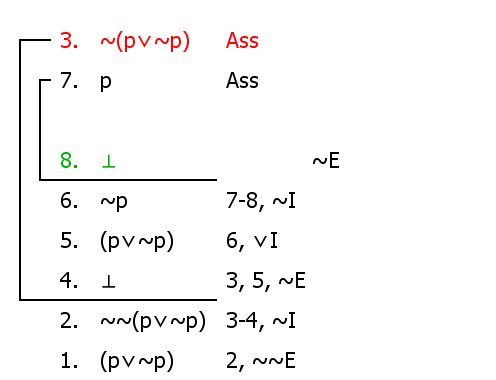
\includegraphics[width=.50\textwidth]{images/save.png}
	\caption{Example of exported \texttt{.png}}
	\label{fig:save}
\end{figure}


\subsubsection{Export to \texttt{.gif}}
This will export the current proof to an animated \texttt{.gif} file. Each step in the proof (up to the current state of the proof) will be given one second in the animation. The final state will be given three seconds. If you have undone any of the proof, all of the redos will be included. You must choose where to save the file.



\subsubsection{Copy proof to clipboard}
This copies a transparent image of the current proof state to the clipboard. Note: this feature does not work well, and does not seem to work at all on OSX.

\subsection{Save and Open}
You can save any proof to a \texttt{.ndp} or \texttt{.ndu} file and open such files. The undo/redo history is saved with the proof, as is the arity list, the current ruleset and the current preset name.

A \texttt{.ndp} file is an editable proof file. You can make changes to these files. A \texttt{.ndu} file is uneditable. Opening such a file will cause ``forward'' and ``back'' buttons to appear above the Proof Panel. Use these to move through the proof.

\begin{figure}
	\centering
		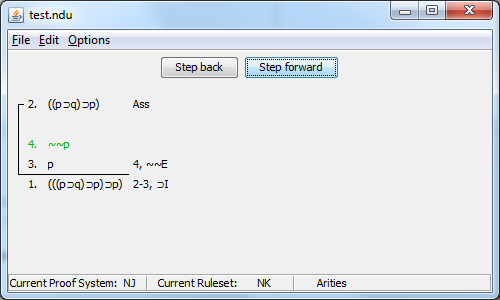
\includegraphics[width=0.70\textwidth]{images/ndu.png}
	\caption{An opened \texttt{.ndu} file.}
	\label{fig:ndu}
\end{figure}


\subsection{Further Features}
There are a number of further features you may wish to use. They are summarised here.

\begin{description}
	\item[Cut Line] Cut\index{Cut} line allows you to insert a new line into the proof. It can be found under \emph{Edit}. The new line will be placed immediately above the current goal.
	\item[Reverse the order of 2-place introductions] This\index{Reverse the order of 2-place introductions} option reverses the order in which two place introduction rules (like conjunction introduction) create lines.
	\item[Show lines in scope of goal] This\index{Show lines in scope of goal} feature causes lines out of scope of the current goal to be displayed in grey, rather than the normal black.
	\item[Zoom] Zoom\index{Zoom} can be controlled from the \emph{Options} menu. The slider in the \emph{Zoom} dialog moves in increments of 50\% - the first mark is 50\% and the final is 550\%. You can increase/decrease the zoom beyond these using \emph{Zoom in} and \emph{Zoom out} in the \emph{Options} menu.
\end{description}

\section{Input Style}
\label{sec:InputStyle}\index{Input}
This section will discuss the best style to use to ensure the Proof Assistant correctly parses your input. For the this section, we will use the following paradigm:

\begin{table}[htbp]
\begin{tabular}{l p{9cm}}
;S; & The symbol that we are considering. This could be $\&$, $\sim$, $\exists$... \\
;argument; & An argument of an operator. There could be more than one of these. This could be a propositional variable, a formula, a term... \\
;argumentX; & where ;X; is an integer. The ;X;th argument.
\end{tabular}
\end{table}

\subsection{Unary Operators}
There are a number of types of unary operators. In general, input a unary operator in the format

\begin{center}
;S(argument);
\end{center}

However, in some cases (such as when the ;argument; contains no further operators) you may leave out the brackets.

Special cases of unary operators are documented in the following sections.

\subsubsection{Quantifiers, @, $\downarrow$}
Quantifiers, @ and $\downarrow$ all behave in the same way. You can use one of the following formats:
\begin{center}
;Sargument1(argument2);
\end{center}

\begin{center}
;S(argument1)(argument2);
\end{center}
where ;argument1; is the variable quantified/term and ;argument2; is the main argument of the operator. If ;argument2; has no further operators, or the next operator is a quantifier, you can use the format ;Sargument1 argument2;.
\subsubsection{[], $\langle \rangle$}
[] and $\langle \rangle$ use the same format. They can be inputted in the following ways.

For [],
\begin{center}
;[argument1](argument2);
\end{center}

For $\langle \rangle$,
\begin{center}
;<argument1>(argument2);
\end{center}
where ;argument1; is the term internal to the operator and ;argument2; is the main argument of the operator (e.g. in $[r]p$, $r$ is ;argument1; and $p$ is ;argument2;). If ;argument2; has no further operators, you can use the format ;[argument1]argument2; or ;<argument1>argument2;.

\subsection{Binary Operators}
For binary operators, you need to use brackets. In general, you must use the following format.

\begin{center}
;(argument1Sargument2);
\end{center}
where ;argument1; and ;argument2; are the two arguments of the operator. 

\subsubsection{Identity}
For identity, you may choose whether or not to surround your terms with brackets.

\subsubsection{Arithmetic}
You do not need brackets around multiplication or addition - these will be added automatically. However, if a term contains more than one of these operators, you will need brackets to specify the order of operations.

\subsection{Predicate Symbols and $n$-ary Functions}
You do not need brackets for $n$-ary functions. You may use them for ease of input if you wish. The arity of each function symbol is determined by the arities list, and not by the location of your brackets (which will be removed). You may also use commas, which will be ignored.

The same situation occurs with Predicate Symbols. You do not need brackets or commas. You can input them, but they will be ignored. You do not need to specify the arity of predicate symbols - this information is not used.


\section{Advanced Usage}
This section will cover more advanced features. It is assumed the reader has read Section \ref{sec:BasicUsage}.

\subsection{GUI Features}
This section complements Section \ref{subsec:ProgramLayout}.

\subsubsection{Status Bar}
As you will have seen, the status bar shows the current ruleset and a label \emph{Arities}, each of which can be clicked to open the \emph{Rule Palette} and \emph{Settings}, respectively. 

The tooltip on the \emph{Arities}\index{Arity List} label gives information on the currently used and unused arities set. If an arity has been used \emph{in a rule application}, it is moved to the used list. Otherwise, it remains on the unused list.

The status bar also contains a label for the \emph{Current Proof System}. This is determined by finding the weakest rule preset that supports all of the currently used rules. This may differ from the current ruleset. If the current ruleset is Q, but all we have used is conjunction introduction, then the current proof system will probably be NJ. If we've specified a custom preset called F, which contains only the rule conjunction introduction, then the current proof system will be F, as this is weaker than NJ but supports all rules used in the current proof. If there is more than one weakest system then all appropriate weakest systems are displayed.

At the far right of the status bar, generally hidden, is the number of the Q axiom currently selected, if it has been selected via the keyboard.

\subsection{New Proof}
Here we will discuss some advanced features of the \emph{New Proof} dialog.

\subsubsection{Numbers for Q}
In Q, we use a unary function symbol ;S; to stand for \emph{successor}. The arity list contains ;S1; by default, and you can input numbers in the format ;SSSS0;.

You are also able to input digits for numbers. These will be converted to the appropriate ;SS...S0;. To see digits rather than ;SS...S0; in the proof itself, select the checkbox marked \emph{Show numbers in Robinson Arithmetic}\index{Show numbers in Robinson Arithmetic} in the \emph{Settings} dialog.

\subsection{New Proof from {\TeX} Code}
You are able to create a new proof from {\TeX} code by selecting the item under \emph{File}, \emph{Advanced}.

You can input sequents here using the same format as the \emph{Output to {\TeX} Code}. Separate formulas by commas and remember to use \emph{->} to flag the conclusion. 

You can input digits for numbers, as with the standard \emph{New Proof}. ;\ul{1}; will also work for ;S0;, ;\ul{2}; for ;SS0; and so on.

\subsection{Output to {\TeX} Code}
This feature is found under \emph{File}, \emph{Export}. You can use it to export to an \texttt{NDProof} environment as defined in \texttt{ndproof.sty}. For the {\TeX} code to be successful, you need to import \texttt{ndproof.sty} and \texttt{mylogicv03.sty}.

\subsection{Command Line Arguments}
You can launch the Proof Assistant from the command line with no arguments. This achieves the same result as simply launching the JAR file. You can also, however, use command line arguments.

\subsubsection{One Argument}
You can supply the name/location of a \texttt{.ndp} or \texttt{.ndu} file to be opened as a single command line argument.

If you supply exactly one command line argument, it will always be assumed that this is a \texttt{.ndp} or \texttt{.ndu} file. If it is not, an error will be given and the Proof Assistant will start as if no arguments were given.

\subsubsection{Two or More Arguments}
You can supply a sequent to start the app with as a series of command line arguments. This must be in the same format as \emph{New Proof from {\TeX} Code}. Remember to flag the conclusion (thus ensuring there will always be at least two arguments).

Tip: If you're not sure what the input {\TeX} should look like, create the proof you want using the friendly \emph{New Proof} and then export to {\TeX}. Use the result to formulate your sequent.


\section{Experimental Features}

\subsection{Magic Mode}
Magic Mode is a simplistic attempt at automatic proof solving. Select a current goal and a current resource and magic mode will apply every automatic rule it can, until it reaches a choice or 10 rule usages. This feature is experimental.

\printindex
\end{document}